%%
%% This is file `sample-authordraft.tex',
%% generated with the docstrip utility.
%%
%% The original source files were:
%%
%% samples.dtx  (with options: `authordraft')
%% 
%% IMPORTANT NOTICE:
%% 
%% For the copyright see the source file.
%% 
%% Any modified versions of this file must be renamed
%% with new filenames distinct from sample-authordraft.tex.
%% 
%% For distribution of the original source see the terms
%% for copying and modification in the file samples.dtx.
%% 
%% This generated file may be distributed as long as the
%% original source files, as listed above, are part of the
%% same distribution. (The sources need not necessarily be
%% in the same archive or directory.)
%%
%% The first command in your LaTeX source must be the \documentclass command.
\documentclass[sigconf, authordraft]{acmart}

%%
%% \BibTeX command to typeset BibTeX logo in the docs
\AtBeginDocument{%
  \providecommand\BibTeX{{%
    \normalfont B\kern-0.5em{\scshape i\kern-0.25em b}\kern-0.8em\TeX}}}

%% Rights management information.  This information is sent to you
%% when you complete the rights form.  These commands have SAMPLE
%% values in them; it is your responsibility as an author to replace
%% the commands and values with those provided to you when you
%% complete the rights form.

%% These commands are for a PROCEEDINGS abstract or paper.


%%
%% Submission ID.
%% Use this when submitting an article to a sponsored event. You'll
%% receive a unique submission ID from the organizers
%% of the event, and this ID should be used as the parameter to this command.
%%\acmSubmissionID{123-A56-BU3}

%%
%% The majority of ACM publications use numbered citations and
%% references.  The command \citestyle{authoryear} switches to the
%% "author year" style.
%%
%% If you are preparing content for an event
%% sponsored by ACM SIGGRAPH, you must use the "author year" style of
%% citations and references.
%% Uncommenting
%% the next command will enable that style.
%%\citestyle{acmauthoryear}

%%
%% end of the preamble, start of the body of the document source.
\begin{document}

%%
%% The "title" command has an optional parameter,
%% allowing the author to define a "short title" to be used in page headers.
\title{CS474 term project paper}

%%
%% The "author" command and its associated commands are used to define
%% the authors and their affiliations.
%% Of note is the shared affiliation of the first two authors, and the
%% "authornote" and "authornotemark" commands
%% used to denote shared contribution to the research.
\author{Jihee Park}
\affiliation{%
  \institution{KAIST}
  \city{Daejeon}
  \country{Korea}
}
\email{webmaster@kaist.ac.kr}

\author{Junseop Ji}
\affiliation{%
  \institution{KAIST}
  \city{Daejeon}
  \country{Korea}}
\email{larst@kaist.ac.kr}

\author{Soyoung Yoon}
\affiliation{%
  \institution{KAIST}
  \city{Daejeon}
  \country{Korea}
}
\email{abc@kaist.ac.kr}
%%
%% The abstract is a short summary of the work to be presented in the
%% article.
\begin{abstract}
  Due to the massive increase of news articles in the internet,
  the importance of topic analysis and issue tracking is growing.
  However, the massive amount of data makes people hard to do the work manually,
  so the automatic process held by the machine is needed.
  In this paper, we suggest an automatic news analysis process, which consists three steps:
  \textit{1. trend analysis}, \textit{2. on-issue event tracking}, and \textit{3. off-issue event tracking}.
  For trend analysis, we use LDA with NER promotion, and for on-issue and off-issue tracking,
 we use DBSCAN and several libraries. 
 After the experiment, we see that our trend analysis model clusters the news articles by topics
  very well, and event tracking models find out the events for each issue(topic).
  our code can be found on the github repository.
  \footnote{https://github.com/soyoung97/Topic\_modeling-Issue\_Tracking}
\end{abstract}
%%
%% Keywords. The author(s) should pick words that accurately describe
%% the work being presented. Separate the keywords with commas.
\keywords{topic modeling, event tracking, news analysis}



%% A "teaser" image appears between the author and affiliation
%% information and the body of the document, and typically spans the
%% page.

%%
%% This command processes the author and affiliation and title
%% information and builds the first part of the formatted document.
\maketitle
\nocite{*} %% temporary nocite
\section{Introduction}
Lorem ipsum dolor sit amet, consectetur adipisicing elit, sed do eiusmod
tempor incididunt ut labore et dolore magna aliqua. Ut enim ad minim veniam,
quis nostrud exercitation ullamco laboris nisi ut aliquip ex ea commodo consequat.
Duis aute irure dolor in reprehenderit in voluptate velit esse cillum dolore eu 
fugiat nulla pariatur. Excepteur sint occaecat cupidatat non proident,
sunt in culpa qui officia deserunt mollit anim id est laborum.


\section{Overview}
Lorem ipsum dolor sit amet, consectetur adipisicing elit, sed do eiusmod
tempor incididunt ut labore et dolore magna aliqua. Ut enim ad minim veniam,
quis nostrud exercitation ullamco laboris nisi ut aliquip ex ea commodo consequat.
Duis aute irure dolor in reprehenderit in voluptate velit esse cillum dolore eu 
fugiat nulla pariatur. Excepteur sint occaecat cupidatat non proident,
sunt in culpa qui officia deserunt mollit anim id est laborum.


\section{Trend analysis}
\usepackage{minted}

\subsection{Data Preprocessing}
\subsubsection{Data Format}
As described in the READ.ME of data provided, The targeted data is from the Korean Herald, National Section news. The period of the dataset is from 2015 to 2017. The Crawled date of the dataset is 2018-10-26. Data format is Json, and there are total of 6 data headers - title, author, time, description, body, and section. Total of 23769 news are included in this dataset.
\subsubsection{Load Data}
In order to load the data, the instructions recommended at READ.ME are followed. Pandas library is used for better storing and access of the news text.
\subsubsection{Libraries Used}
For this project, we used pandas and gensim python libraries.


\subsection{Previous approaches}
Issue trend analysis can be seen as a part of Topic modeling. By searching fields of recent Topic modeling, LDA has shown to have good performance. As a result, LDA is used as a baseline algoritm for this project.
A recent study(2018) on Topic Modeling shows that Topic Quality improves when Named Entities are promoted.\site{krasnashchok-jouili-2018-improving} This paper proposes 2 techniques: 1.Independent Named Entity Promoting and 2.Document Dependent Named Entity Promoting. Independent Named Entity Promoting promotes the importance of the named entities by applying scalar multiplicaion alpha to the importance of the named entity word. Document Dependent Named Entity Promoting promotes the importance of the named entities by setting the weights of the named entities as maximum term-frequency per document. For Independent Named Entity Promoting, the value of alpha can be changed flexibily, but results conducted by this paper shows that setting alpha as 10 showed the best results.
We take advantage of this paper and implement Named Entity Promoted Topic Modeling done by LDA.
\subsection{Experiments}
\subsubsection{Data Tokenization}
\subsubsubsection{Lemmatization is not always good}
At first try, Lemmatization(converting words into base forms) and removal of stopwords were conducted before we run the LDA algorithm and extract Named Entities. We thought that converting words into base forms and reducing the total vocabulary size would increase the performance of topic modeling. Stopwords were taken from \mintinline{python}{nltk.corpus.stopwords.words("english")}, and lemmatization functon was taken from \mintinline{python}{gensim.utils.lemmatize}. \mintinline{python}{res.append(lemmatize(raw\_text, stopwords=stopwords))}. But after we do lemmatization, remove stopwords, and tokenize the data, no Named Entities were extracted from the preprocessed corpus. We think the reason for this is as follows. 
First, words are all converted into lower case when we do lemmatization. This makes the Named Entitiy Recognition system(NER system) to work poorly because we have removed the original information whether the word has a high probability that it is a "Proper pronoun" or not.(고유대명사).
Second, words are transformed into their base forms, limiting NER system to detect specific words. There also could be cases that the words are transformed into meanings other then their original meanings. For example, "Cooking" and "Cooker" are both converted into "cook" when they are lemmatized, and this makes the word to lose the original information.
Third, original relationships between words are lost, because of the removal of stopwords. When we do NER, we have to do the POS tagging of the sentence and then input both the word sequence and the POS sequence of the text. But when we artificially remove stopwords and then do NER, original relationships between words are disrupted and broken. This limits NER system to perform well.

For these 3 reasons, we decided to NOT apply lemmatization for tokenization, because lemmatization lose so much information about the original text and disrupts the NER system's ability to detect
 Named Entities properly. We decided to just do POS tagging and then do NER. We just used word\_tokenize from nltk.tokenize.

\subsubsection{Extract NER}
By using ne\_chunk from nltk and pos\_tag from nltk.tag, we extracted Named entities from the original news dataset. NER also extracts multi-word information of Named Entities other than just class
ifying whether a word is a named entity or not, so we decided to use that information. We store single-word Named Entities and multi-word named entities separately. As a result, NER and multi-wor
d extraction of NER are both processed.

below figure is the topic modeling result(of all time lengths from 2015 to 2017) WITH NER Promoting and WITHOUT NER Promoting. We can see the difference between those two results, and we can conc
lude topic modeling with NER promoting shows better performance.
\begin{figure*}[t]
    \centering
\includegraphics[width=0.8\textwidth]{afterner.png}
\includegraphics[width=0.8\textwidth]{beforener.png}
\end{figure*}
\subsubsection{Do LDA}
At first try, we ran LDA on naive ner boosted news dataset. but with this approach, we found out that stopwords are classified as top(important)words according to the result of LDA. So we decided to remove stopwords after all the preprocssing(including NER weight promoting)are done. The timing of removal of stopwords are important, as removing stopwords before NER will affect the NER result. Stopword removing are done right before feeding the tokens into LDA. After the removal of stopwords, we could see that the results were much better.

\subsubsection{Apply neuroNER} 
On the topic modeling paper that we referenced says that it uses neuroNER. neuronNER is an easy-to-use program for named entity recognition based on neural networks presented in emnlp 2017. \site{2017neuroner} This neuroNER tool is trained on CONLL2003 dataset and recognizes four types
of NE: person, location, organization and miscellaneous. Instead of using \mintinline{python}{ne_chunk(pos_tag(preprocessed_text), binary=True)}, we use
\begin{minted}{python}
nn = neuromodel.NeuroNER(train_model=False, use_pretrained_model=True)
nn.predict(preprocessed_text)
\end{minted}
to extract Named Entities from the text.


\subsubsection{Do LDA with NER promoting.}
First, split the dataset each year. Then, get tokens for each document with promoted NER frequency (X 10). With this corpus, run the LdaModel with num\_topics of 10 and num\_words of 30 to 50.
\subsubsubsection{Tuning LDA hyperparameters}
At first, we decided to train the LDA model with num\_topics of 10 and num\_words of 15. But the results were not very explainable. After experimenting with num\_topics and num\_words, we found that setting num\_topics of 10 is the best representative of the total news. Also, since the only removed word was the stop word, non-ascii character, or unrelated words such as \mintinline{python}{" \xec ' ( ) . ,} were introduced in the topic result. To extract useful information, we increased num\_words for each topics to 50.



\section{On-issue tracking}

For on-issue tracking, we first divide news articles monthly.
Then we classify news articles in each month group into 10 issue categories.
For each classified group, each article’s 5W1H(when, where, who, what, why, how) is extracted and counted.
The frequencies are used to extract the most relevant news title for each month.

Figure \ref{fig:onissuedia} shows the structure of the on-issue tracking process.

\begin{figure}[!htbp]
  \centering
  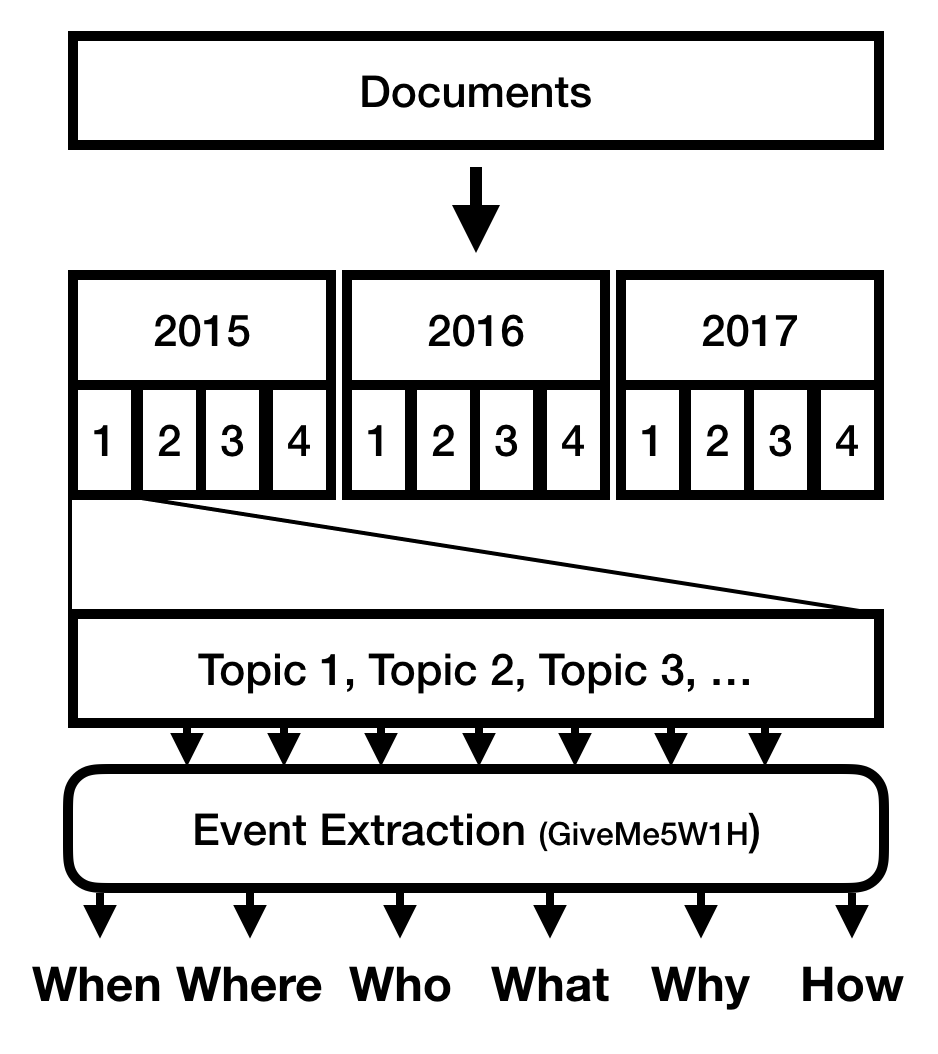
\includegraphics[width=0.8\linewidth]{on_issue_1.png}
  \caption{A brief diagram of on-issue tracking process.}
  \label{fig:onissuedia}
\end{figure}

\subsection{Monthly Division}

We divided all news articles monthly.
The groups contain news articles those are written in \textit{January 2015, Febuary 2015, \dots, December 2017, January 2018}.
\textit{2018 Jan.} group contains only a few articles,
so we decided to ignore the last group.
The reason why we divided the data monthly is, the month is one of the standard in the field of yearly statistics analysis.
For example, the issue about MERS started from May 2015, and ended in January 2016.
If we divide yearly, there will be only one or two groups for extracting events.
Else if we divide quarterly, there will be three or four events.
We can extract eight or nine events from the period if we divide the events mothly,
so this is just fit to make a reasonable result.

\subsection{Articles in the Months Categorization}

With LDA model we have trained at trend analysis project,
we classify the documents in the month groups.
If we give a tokenized sentence to the LDA model,
the model outputs the probability for each group.
We choose the group with maximum value, and assign the document to the group.
So, for each month, there are 21 classified groups of news articles.

\subsection{Event Extraction}

For each group we divided from above,
we extract the events with the approach of word frequency.
For this step, we use a Python library called ``giveme5W1H''\cite{Hamborg2019b}.
The library is the state-of-the-art tool for extracting
\textit{when/where/who/what/why/how} features from the document.
The library uses Stanford's CoreNLP library as its basic structure,
and give analysis results when we give a
title, lead, text, and a published date.
We decided to use columns \textit{title}, \textit{description}, \textit{body}, and a \textit{time}
from the given dataset as an input to get a result.
For each group, we count the frequencies of each feature of the articles,
and select the most frequent terms for each feature, treat them as a score.
Then we extract a most relevant article from the monthly group;
For example, if the term `president' occurs twelve times and
`government' occurs six times as \textit{Who} feature,
the news article contains the term `president' as \textit{Who}
takes double scores than the the article about `government'.
The maximum score article's headline is assumed that it is
representing the main event of the month.

We choose two yearly issues from the list, and do event extraction for each issue.
For each month result, we identify an event based on the result and align them on the timeline.

Table \ref{table:onissue} is an example of on-issue tracking of the issue MERS.

\begin{table}[!htbp]
  \begin{tabular}{l|l}
  Month   & Event(headline)                                        \\ \hline
  2015.06 & S. Korea confirms 3 more MERS cases, total rises to 18 \\
  2015.07 & S. Korea reports no new MERS cases for 17th day        \\
  2015.08 & Park gives appointment letter to new health minister   \\
  2015.09 & Moon stakes leadership on party reform                 \\
  2015.10 & 61 isolated after last MERS patient rediagnosed       
  \end{tabular}
  \caption{The example of on-issue tracking of the issue MERS.}
  \label{table:onissue}
\end{table}
\section{Off-issue tracking}
For off-issue tracking, we first categorize topics given as Trend analysis part.
In this section, we denote a document as sequence of tokens plus its created time $\mathbb{D} := (\Sigma^{+}, t)$, when $t \in \mathbb{R}$ (timestamp of creation time).
and the set of document of topic $a$ as $\mathbb{T}_{a} \in \mathcal{P}(\mathbb{D})$.

\subsection{BoW extractuion}
In first, we have to extract document in some space which we can analyze quantatively.
We use BoW as morphism from document space to vector space $\mathbb{R}^{N}$, which we can
analyze similarity of document. In addition, we add one more dimension to give information
of document creation time. From pre-calculated set of tokens $\Sigma := \{ \sigma_{1}, \sigma_{2}, \ldots, \sigma_{n} \}$,
our transformation $b: \mathbb{D} \rightarrow \mathbb{R}^{n+1}$ is defined inductively as
\[
\begin{cases}
    b([], t) := t * e_{n+1}\\
    b(\sigma_{i} :: tl, t) := e_{i} + b(tl, t)
\end{cases} 
\]
Then, morphism from $\mathbb{T}_{a} \in \mathcal{P}(\mathbb{D})$ to $\mathcal{P}(\mathbb{R}^{n+1})$ is naturally induced from $b$ as
$\phi(\mathbb{T}_{a}) = \{b(d) | d \in \mathbb{T}_{a}\}$

\subsection{Relation between semantic of document and BoW}
We know that there are documents and events which have similar meaning, but we cannot formalize it because we currently do not have
model of language interpretation in metric space. But we can assume \textit{such} space exists, i.e. there is an isomorphism
$\phi: \mathbb{D} \rightarrow \mathbb{D}^{\#}$, when $(D^{\#}, d^{\#})$ is metric space. It is not hard to assume this structure,
since similar concept is already introduced as Entity comparison/Behavior comparison operator of Semantic algebra \cite{wang2013semantic}.

Our desired result is that $b$ with euclidean distance successfuly models $(D^{\#}, d^{\#})$, but we cannot show it because we do not have
constructive definition of $D^{\#}$. But if it has sufficient approximation, (bounded approximation)
We can derive more interesting properties (such as bounded error from BoW to Event space, etc).

\begin{definition}
    $b$ has approximation of $\phi$ with bound $K, \epsilon$ iff there exists an Lipshitz continuous $\pi$ with $K$ that $d^{\#}(\pi(b(d)), \phi(d)) \leq \epsilon$.
\end{definition}

\subsection{Relation between semantic of event and BoW}
Once semantic of document is defined, we can build similar notion of event as metric space. To build such space, we first understand about
relation between document and event.
\begin{itemize}
    \item similar document refer similar event.
    \item similar event (even same event) may be refered by documents with far distance, but it is not arbitrarly far.
\end{itemize}
we can formulize this as logical formlua, with definition of $e: D^{\#} \rightarrow E^{\#}$. ($(E^{\#}, e^{\#})$ is metric space for event)
\begin{itemize}
    \item if $d^{\#}(d_{1}, d_{2})$ is sufficiently small, then $e^{\#}(e(d_{1}), e(d_{2}))$ is sufficiently small.
    \item when $e^{\#}(e(d_{1}), e(d_{2}))$ is small, it doesn't mean $d^{\#}(d_{1}, d_{2})$ is small but is bounded.
\end{itemize}
begin with this fact, we can find very interesting property which generalize this: continuity.
\begin{definition}
    $e$ is Lipschitz continuous with $K$ if and only if\\ $e^{\#}(e(d_{1}), e(d_{2})) \leq K d^{\#}(d_{1}, d_{2})$.
\end{definition}

We can check that if $e$ is Lipschitz continuous with $K_{e}$, then above two property is satisfied. Also, it derives important fact:
If we have approximation of semantics with bounded error, then there also exists approximation of event with bounded error.
\begin{theorem}
    $b$ has approximation of $\phi$ with bound $K, \epsilon$, then there exists $\pi_{e}: \mathbb{R}^{n+1} \rightarrow E^{\#}$ s.t.
    $e^{\#}(\pi_{e}(b(d)), e(\phi(d))) \leq K_{e} \cdot \epsilon$. (it means $b$ has approximation of $e \cdot \phi$ with bound $K, K_{e} \cdot \epsilon$)
\end{theorem}
Although proof is directly derived from Lipschitz continuity, it emphasizes that if we have bounded approximate of document, then it guarantees
bounded approximation of event.

\subsection{Event clustering}

In this assumption about semantic of document ans event, we can build event clustering method. Before using techniques in $R^{n+1}$, we
focus on how this clustering in $R^{n+1}$ effects in $E^{\#}$.

\begin{theorem}
    if $b$ has approximation of $e \cdot \phi$ with bound $K, \epsilon$, then $e^{\#}(e \cdot \phi(d_{1}), e \cdot \phi(d_{2})) \leq 2 \cdot \epsilon + K || b(d_{1}) - b(d_{2}) || $.
\end{theorem}

\begin{proof}
    \begin{align*}
     & e^{\#}(e \cdot \phi(d_{1}), e \cdot \phi(d_{2})) \leq e^{\#}(e \cdot \phi(d_{1}), \pi_{e}(b(d_{1}))) + \\
     & e^{\#}(\pi_{e}(b(d_{1})), \pi_{e}(b(d_{2}))) + e^{\#}(\pi_{e}(b(d_{2})), e \cdot \phi(d_{2})) \leq \\
     & \epsilon + e^{\#}(\pi_{e}(b(d_{1})), \pi_{e}(b(d_{2}))) + \epsilon \leq \\
     & 2 \cdot \epsilon + K || b(d_{1}) - b(d_{2}) ||.
    \end{align*}
\end{proof}

It shows that, if we make good Vector transformation $b$, then it automatically guarantees bounded error for distance of extracted event, without
construction of $\pi$, $\phi$, $e$ or any other. Begin with this fact, we derive constructive definition of partition for documents using approximated
transformation $b$. To do that, we first define similarity for two documents.

\begin{definition}[Similarity relation]
    $\approx_{\mathbb{R}^{n+1}, \delta} \in \mathcal{P}(\mathbb{D \times D})$ is defined as \begin{displaymath}
        d_{1} \approx_{\mathbb{R}^{n+1}, \delta} d_{2} \Longleftrightarrow || b(d_{1}) - b(d_{2}) || \leq \delta.
    \end{displaymath}
    Similarly, $\approx_{E^{\#}, \delta} \in \mathcal{P}(\mathbb{D \times D})$ is defined as \begin{displaymath}
    d_{1} \approx_{E^{\#}, \delta} d_{2} \Longleftrightarrow e^{\#}(e \cdot \phi(d_{1}), e \cdot \phi(d_{2})) \leq \delta.
    \end{displaymath}
\end{definition}
then $\approx_{\mathbb{R}^{n+1}, \delta} \subseteq \approx_{E^{\#}, 2 \cdot \epsilon + K \cdot \delta}$ holds by above theorem. Thus it is quite
reasonable to use $\approx_{\mathbb{R}^{n+1}, \delta}$ to cluster events.

\begin{definition}[Transitive closure]
    $\approx_{\mathbb{R}^{n+1}, \delta}^{*}$ is smallest relation on $\mathbb{D}$ that contains $\approx_{\mathbb{R}^{n+1}, \delta}$ and is transitive.
\end{definition}

Then $\approx_{\mathbb{R}^{n+1}, \delta}^{*}$ is reflexive, symmetric and transitive, which can be equivalence relation. Then, we can partition
documents with this equivalence relation.

\begin{definition}[Partiton of $\mathbb{D}$]
    when $\approx$ is equivalence relation, $\mathbb{D}/\approx := \{[a] | a \in \mathbb{D}\}$, when $[a] := \{b \in \mathbb{D} | a \approx b \}$.
\end{definition}

By substitute $\mathbb{D}$ to $\mathbb{T}_{a}$, finally we have $\mathbb{T}_{a}/\approx_{\mathbb{R}^{n+1}, \delta}^{*}$ as successful approximation 
of event partition of topic $a$. Now, we are going to explain how most relevent description of event is extracted from each partiton.
\section{Evaluation}

\subsection{Trend analysis evaluation}
To evaluate our result, we first try to show that our trend analysis
works well. To do that, we collect other document with topic label.
With these test set, its trend analysis result indirectly shows our
accuracy of trend analysis.
\subsection{Selecing test set}
We use reuters data set. It consists of more than 9000 documents
with more than 70 topics. But, the similairty of document is important
because evaluation on very diffrent set of doucments dosen't imply
any meaningful result. To resolve that, we decided to extract 10 topics
with most similairty between our dataset. It is achived by calculating
document similarity between reuters dataset and our news dataset.

To pick most similar topic, we compute maximum similairty within documents
in topic and minimum similairty bewteen reuters and news dataset. Due to
largeness of dataset, we choose only subset of dataset to calculate
minimum/maximum similairty bewteen groups.

\subsection{Reuters evaluation}
With reuters dataset with 10 pre-classified topics, we generate LDA
model for reuters dataset and make 10 topics. And we classified the topic
with given label. In result, we successfuly classified 7 topics from
LDA result. It shows that our LDA model seems to work correctly.

\section{Conclusion}
Lorem ipsum dolor sit amet, consectetur adipisicing elit, sed do eiusmod
tempor incididunt ut labore et dolore magna aliqua. Ut enim ad minim veniam,
quis nostrud exercitation ullamco laboris nisi ut aliquip ex ea commodo consequat.
Duis aute irure dolor in reprehenderit in voluptate velit esse cillum dolore eu 
fugiat nulla pariatur. Excepteur sint occaecat cupidatat non proident,
sunt in culpa qui officia deserunt mollit anim id est laborum.


%%
%% The acknowledgments section is defined using the "acks" environment
%% (and NOT an unnumbered section). This ensures the proper
%% identification of the section in the article metadata, and the
%% consistent spelling of the heading.

%%
%% The next two lines define the bibliography style to be used, and
%% the bibliography file.
\bibliographystyle{ACM-Reference-Format}
\bibliography{report}
\end{document}
\endinput
%%
%% End of file `sample-authordraft.tex'.
